\documentclass[12pt]{article}
\usepackage[a4paper, margin=1in]{geometry}
\usepackage{graphicx}
\usepackage{float}
\usepackage{hyperref}
\usepackage{listings}
\usepackage{color}
\usepackage{amsmath}
\usepackage{fancyhdr}
\usepackage{caption}
\usepackage{enumitem}
\usepackage{titlesec}

\pagestyle{fancy}
\fancyhf{}
\rhead{COMP1610 Coursework}
\lhead{Greenwich Bank}
\rfoot{Page \thepage}

\titleformat{\section}{\Large\bfseries}{\thesection}{1em}{}

\title{COMP1610 Coursework Report \\ \large Programming Enterprise Components \\ \large \textbf{Bank App Project}}
\author{Jack Jibb\\ 001408490 \\ Other Group Members: \\ Syed Ali Irtaza – 001414068 \\ Anastasiia Pyslar – 001412071 \\ Devanshi Pandya – 001426270 \\ Poorva Motaval – 001449334  }
\date{Submission Date: 24 March 2025}

\begin{document}


\maketitle
\newpage
\tableofcontents
\newpage

\section{Design Documentation (Group Work)}

\subsection{Entity-Relationship Diagram}

\begin{figure}[H]
	\centering
	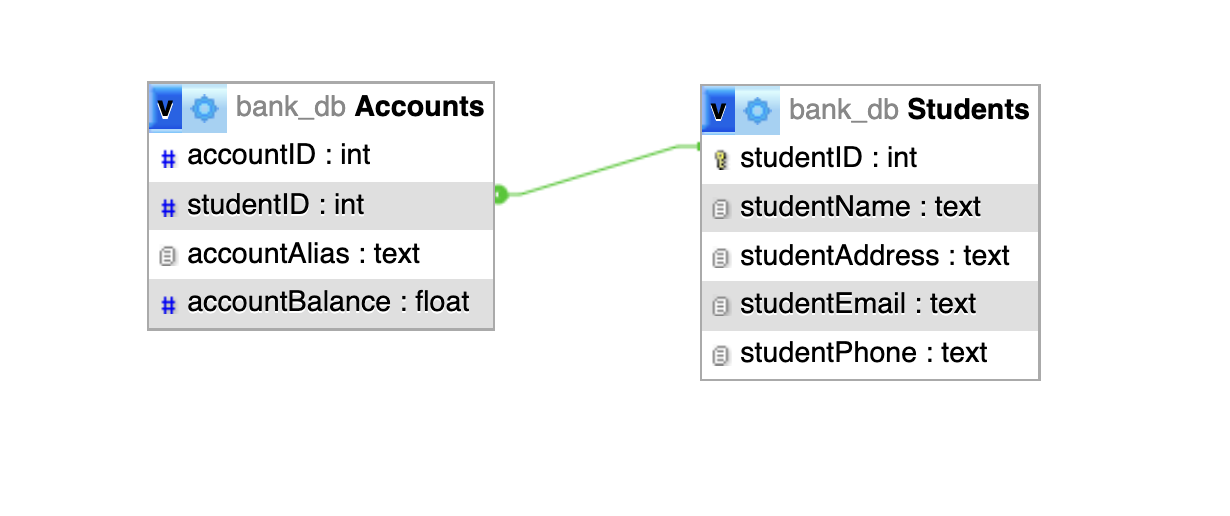
\includegraphics[width=0.5\textwidth]{./assets/ERD}
	\caption{Entity Relationship Diagram for the Database}
\end{figure}

\subsection{Architecture Diagram}

\begin{figure}[H]
	\centering
	\includegraphics[width=\textwidth]{architecture_placeholder.png}
	\caption{Overall Application Architecture}
\end{figure}

\section{Screenshots (Group Work)}
Add one screenshot per implemented feature, e.g., student listing, account creation, transfers.

\begin{figure}[H]
	\centering
	\includegraphics[width=0.8\textwidth]{create_account.png}
	\caption{Create Account Feature}
\end{figure}

\subsection*{Feature List:}

This section outlines the implemented features of the Banking Web Application, categorized by functionality. Each category includes a description and a self-assessment box (1 = Poor, 5 = Excellent) to reflect how well the features were implemented.

\subsubsection{Authentication \& Session Management}

\begin{itemize}
	\item \textbf{Student Login:} Dropdown menu for selecting and logging in a student.
	\item \textbf{Session Cookies:} Username and student ID stored in cookies.
	\item \textbf{Logout:} Clears cookies and session state.
\end{itemize}

\begin{center}
	\fbox{
		\begin{minipage}{0.9\linewidth}
			\textbf{Implementation Rating (1--5):} \underline{4}
		\end{minipage}
	}
\end{center}

\subsubsection{Student Management (CRUD)}

\begin{itemize}
	\item Create student with form (name, email, phone, address).
	\item List all students (admin view).
	\item RESTful API: Create, Read, Update, Delete student.
	\item Cascade delete verified upon student deletion.
\end{itemize}

\begin{center}
	\fbox{
		\begin{minipage}{0.9\linewidth}
			\textbf{Implementation Rating (1--5):} \underline{5}
		\end{minipage}
	}
\end{center}

\subsubsection{Account Management (CRUD)}

\begin{itemize}
	\item Create account (initial balance £0, linked via student ID from cookie).
	\item Conditional listing (all accounts or student-specific).
	\item Detailed view per account with deletion.
	\item RESTful API: Create, Read, Update, Delete account.
\end{itemize}

\begin{center}
	\fbox{
		\begin{minipage}{0.9\linewidth}
			\textbf{Implementation Rating (1--5):} \underline{5}
		\end{minipage}
	}
\end{center}

\subsubsection{Transactions (Deposit, Withdraw, Transfer)}

\begin{itemize}
	\item Deposit and withdraw via dynamic form.
	\item Overdraft protection prevents excessive withdrawal.
	\item Transfer funds between accounts with Student validation.
	\item TransactionResult page displays updated balances and outcome messages.
\end{itemize}

\begin{center}
	\fbox{
		\begin{minipage}{0.9\linewidth}
			\textbf{Implementation Rating (1--5):} \underline{4}
		\end{minipage}
	}
\end{center}

\subsubsection{Front-End Features}

\begin{itemize}
	\item Dynamic page loading using JavaScript and AJAX.
	\item Button and form action binding via \texttt{main.js}.
	\item Confirmation prompts for sensitive actions (e.g., delete).
\end{itemize}

\begin{center}
	\fbox{
		\begin{minipage}{0.9\linewidth}
			\textbf{Implementation Rating (1--5):} \underline{5}
		\end{minipage}
	}
\end{center}

\subsubsection{RESTful API (JSON*)}

\begin{itemize}
	\item JSON-based API for students and accounts.
	\item Endpoints for CRUD operations.
	\item Special endpoints for deposit, withdraw, and transfer.
\end{itemize}

\begin{center}
	\fbox{
		\begin{minipage}{0.9\linewidth}
			\textbf{Implementation Rating (1--5):} \underline{3}
		\end{minipage}
	}
\end{center}

\vspace{1em}
\noindent \textit{*Note:} All JSON endpoints consume and produce data via \texttt{MediaType.APPLICATION\_JSON}.

\subsection{REST API Endpoints}
List of all endpoints and the function they serve:
\paragraph{Student API}
\begin{itemize}
	\item \textbf{GET /api/students}:\textit{getAllStudents()}
	\item \textbf{GET /api/students/{student\_id}}:\texttt{getStudentByID(student\_id)}
	\item \textbf{POST /api/students}:\texttt{createStudent(Student Entity)}
	\item \textbf{PUT /api/students}:\texttt{updateStudent(Student entity)}
	\item \textbf{DELETE /api/students/{student\_id}}:\texttt{deleteStudent(student\_id)}
\end{itemize}
\paragraph{Account API}
\newpage
\section{Evaluation (Group Work)}


\section{Research (Individual)}


\section{Individual Reflection (Individual)}

\newpage
\section{Appendix}

\subsection{Application Screenshots}
\subsubsection{Web App Screenshots}

\begin{figure}[H]
	\includegraphics[width=\textwidth]{./assets/Web1}
	\caption{}
\end{figure}

\subsubsection{CLI Application Screenshots}

\subsection{WildFly 33 Server Configuration}

This section outlines the essential configuration settings from the \texttt{standalone-full.xml} used in the deployment of the WildFly 33 application server.

\subsubsection{Subsystems and Extensions}
The configuration includes a comprehensive set of extensions and subsystems to support a variety of Java EE technologies:
\begin{itemize}
	\item \textbf{EJB, JPA, JSF, JAX-RS:} Enabled via \texttt{org.jboss.as.ejb3}, \texttt{org.jboss.as.jpa}, etc.
	\item \textbf{Security:} Configured through WildFly Elytron with domains \texttt{ApplicationDomain} and \texttt{ManagementDomain}.
	\item \textbf{Clustering and Caching:} Infinispan containers set for EJBs and Web session management.
	\item \textbf{Logging:} Console and periodic file handlers with custom formatters.
	\item \textbf{Data Sources:}
	      \begin{itemize}
		      \item \texttt{BankDS}: MySQL datasource connecting to \texttt{bank\_db} using driver \texttt{com.mysql.cj.jdbc.Driver}.
	      \end{itemize}
\end{itemize}

\subsubsection{Management and Access Control}
\begin{itemize}
	\item Management is accessible via HTTP interface bound to \texttt{management-http} (port 9990).
	\item Role-based access is enabled using the \texttt{SuperUser} role mapped to the local user \texttt{\$local}.
	\item Audit logging is available but currently disabled.
\end{itemize}


\subsubsection{Server Interfaces and Socket Bindings}
\begin{itemize}
	\item Interfaces are defined for \texttt{management}, \texttt{public}, and \texttt{unsecure} IP addresses.
	\item Common ports include:
	      \begin{itemize}
		      \item HTTP: 8080
		      \item HTTPS: 8443
		      \item AJP: 8009
		      \item Management HTTP/HTTPS: 9990 / 9993
	      \end{itemize}
\end{itemize}

\subsubsection{Deployment and Monitoring}
\begin{itemize}
	\item Deployment scanner monitors the \texttt{deployments} directory every 5 seconds.
	\item Metrics, health, and microprofile extensions are enabled.
\end{itemize}

\subsubsection{Thread and Resource Management}
\begin{itemize}
	\item Default thread pools are defined for concurrency and EJB processing.
	\item Resource adapters and managed executors are configured under the EE subsystem.
\end{itemize}

This configuration enables a robust and secure environment suitable for enterprise Java applications, with database integration, secure authentication, clustering, and deployment automation.

\subsection{Source Code Structure}
Briefly outline your directory structure:

\begin{verbatim}
BankApp/
│
├── src/
│   ├── controller/
│   ├── dao/
│   ├── model/
│   ├── service/
│   └── rest/
├── webapp/
│   ├── jsp/
│       ├── accounts/
│       ├── home/
│       ├── students/
    │   └── transactions/
│   ├── css/
│   └── js/
└── META-INF/
\end{verbatim}

\subsection{References}
\begin{itemize}
	\item Jakarta EE Documentation: \url{https://jakarta.ee}
	\item WildFly Docs: \url{https://docs.wildfly.org}
	\item MySQL Documentation: \url{https://dev.mysql.com/doc/}
\end{itemize}

\end{document}

